\chapter{Communication}\label{cha:communication}

The goal of the project is to provide a teleoperated surgical system which makes the surgeon controlling the robot feel as if he was manipulating the end-effector directly. To achieve this, the time delay of the force between the end-effector and the controller should be unnoticeable. The targeted communication frequency of 1 kHz should result in a delay small enough to satisfy this need.

\section{Communication between ROS and the sbRIO board}

In the former system setup the sbRIO board and the computer running ROS communicated through a TCP/IP protocol. TCP/IP is a connection orientated protocol, which first establish the connection between two devices. After the connection has been established data can be send in both directions. TCP/IP is a reliable protocol which ensure that the data transmitted, will be received. When the data is send, the transmitter waits for an acknowledgment from the receiver that the data has been received. If the data has been corrupted or the acknowledgment is not send, the transmitter will retransmit the package again. If the case of no acknowledgment is happening, a timer is used to define when to retransmit the data again. The data will then be retransmitted a certain amount of times until an acknowledgment has been received or the connection is defined to be disconnected. This means that a copy of the data is stored at the transmitter until it has been correctly received or the connection is taken down.\\ 
This communication protocol induces delays in the system as the transmitter has to wait on the acknowledgment that the data has been received before loading new data into the sending buffer. If data has been discarded due to error the transmitter has to retransmit the data again if necessary.  

The speed of the communication between the sbRIO board and the computer running ROS is set to 100 Hz. This was done as a trade off between being fast and for avoiding bugs which where bandwidth related\cite{Chris_Surgical}.

% This frequency was just enough to finish transmitting the data coming from the sensors, as a frequency increase resulted in bugs. To prevent data collision while increasing communication frequency, we can either:

The problem with the communication latency can be solved in different way, where some of them are listed below.

\begin{itemize}
	\item Find a faster communication protocol,
	\item Compress data,
	\item or implement faster hardware.	
\end{itemize}

\section*{User datagram protocol}
UDP communication protocol is a faster way of communicating compared to TCP/IP. It is connectionless which means that it wont establish a connection before sending data. When data is transmitted, new data is loaded into the transmitter buffer and then send when the connection line is free, thus the data is not stored at the transmitter as in TCP/IP. Furthermore the UDP protocol does not wait for an acknowledgment and thereby just sends the data as fast as possible to the specified address.

AS the goal is to reduce latency in the communication between the robot and ROS it has been chosen to go with the UDP protocol as it should be faster than the TCP/IP protocol, however less reliable. Because of the higher data rate, package loss or package error should not become a problem, as a new package is send as soon as possible. Furthermore instead of storing old data at the transmitter which can be obsolete if needed to be resend, as in TCP/IP, UDP will send new data instead.


% TCP/IP is a reliable protocol, but the handshaking protocol it uses causes some further latency. By replacing the TCP/IP protocol with the less reliable UDP protocol (User Datagram Protocol), we can reduce the latency of the system. UDP is lacking the handshaking protocol, thus it is more prone to losing packets. However the communication happens between two nodes without any intermediate router, thus the probability of losing packages at a frequency of 1 kHz is rather small.

\section{Data Compression}

Labview's built in UDP write protocol expects an ASCII format string as data input. ASCII encoding was originally a 7 bit encoding format. The need for an extended character set brought an 8 bit version of ASCII encoding, which is included by Labview. The former Labview code's message format is as follows:

\begin{verbatim}
{"p4_primary":{"position":[6,3,2,3],"velocity":[3,2,3,1],"effort":[4,1,1,1]}}
\end{verbatim}
This illustrate a read out of four different motor values.

To minimize the forwarded data size, first of all we have to get rid of the names of each data. To keep the data readable for the receiver, we can either use a character to separate each segment of data, or we can agree upon a constant size for each segment of data.

The former code encoded each digit of a decimal number as an ASCII character. It means that the number segment only used 10 out of the 256 possible characters. To compress data, we should utilize all the ASCII characters. One way to do it is to make a character store the number as its address in the 8 bit address table. We basically have to convert the numbers to base 256.

We utilized Labview's built in flatten to string node, which basically converts numeric data to the correspondent string. For example, it convert an 8 bit integer to the correspondent ASCII character. If the sbRIO and the PC uses the same encoding, they can basically send bitcode as if it was string then decode it by doing a simple conversion.  \todo{check if the 32 bit float can be substituted with a 16 bit ones}
 
The UDP must send encoder, potmeter and current measurement data from each of the four motors. Each data is represented as a 32 bit float. This adds up to 48 bytes of data to be sent each cycle. The described method sends 48 byte long strings not including the header. The former method sends 67 characters for formatting and naming purposes and 96 bytes of numeric data, assuming each double number is sent in 8 digits. It adds up to 163 bytes.

By removing the names from the string and compressing a data, the string can become 70 shorter, which is a valuable increase in efficiency.



\section{Rewriting the driver}

In order to communicate between ROS and the sbRIO board the university created a ROS node called davinci\_driver. This driver is composed of three parts: the low level driver called sbrio\_driver that communicate directly with the sbRIO board, the high level driver called ros\_driver that handle the communication between the other ROS node and the driver and the middle level driver that allow the communication between the low level driver and the high level one.

\subsection{The original driver}
The low level driver connect to one sbRIO board using a TCP/IP socket and launch a loop in a thread to handle the communication. The data exchange is made using a JSON Stream as described in the previous section. The structure of the code can be seen in figure~\ref{original_driver}.

\begin{figure}
\begin{tikzpicture}

\node[box] (Initialization) at (0,0) {Initialization};
\node[box] (Receive) at ($(0,-2)+(Initialization)$) {Read the data \\if some were received};
\node[box] (Send) at ($(0,-2)+(Receive)$) {Send if the\\ control changed};
\node[box] (Sleep) at ($(0,-2)+(Send)$) {Sleep};
\node[box] (Update_State) at ($(5,0)+(Receive)$) {Update the data\\ available for higher\\level processes};

\draw[->, ultra thick] (Initialization) -- (Receive);
\draw[->, ultra thick] (Receive) -- (Update_State);
\draw[->, ultra thick] (Receive) -- (Send);
\draw[->, ultra thick] (Send) -- (Sleep);
\draw[->, ultra thick] (Sleep.west) -| ++(-2,0) |- (Receive);

\end{tikzpicture}
\caption{Structure of the original sbRIO driver}
\label{original_driver}
\end{figure}

The middle level driver allows the creation of more than one low level driver. Thanks to this it is possible to communicate with more than one arm of the DaVinci Robot at once. It also handles the communication between the high level driver and the low level so that there is no need for the client to acquire mutexes.

The high level driver simply updates the data for the other nodes and transmits the setpoints to be sent.

\subsection{The new driver}

In order to increase the speed of the communication it is necessary for us to write a new driver. As previously explained, the new driver should use UDP instead of TCP/IP as we have no use for old data. It should also transmit the actual data without using a JSON Stream so that the size of each packets is reduced. In addition to those objectives we would like to modify as little as possible the current structure of the ROS node so that we don't have to rewrite the entire system. 
We just defined three goals that need to be fulfilled when writing the new driver. Let's identify those goals with numbers:
\begin{enumerate}
	\item Replace TCP by UDP
	\item Replace the JSON Stream by the numerical values
	\item Modify as little as possible the original driver
\end{enumerate}

The modifications that need to be made in order to carry duty 1. and 2. are related to the communication protocol and the format of the transmitted data which are both handled by the low level driver. In order to fulfill goal 3. we should aim to modify the low level driver only without having consequences on the higher level drivers. This means that the public functions should keep the same prototype and that the format of the data available for them should stay the same (i.e vectors of double). We should also try to keep using the boost library used in the original driver to handle threads and mutexes.

The socket initialization for the UDP protocol is very close to the one made for TCP protocol, thanks to this the establishment of the communication with the sbRIO is similar in both the old and new drivers. However, the UDP being connectionless it is not possible to use the same method as before to read incoming data, i.e it is not possible to look if some new data arrived, with UDP it is necessary to constantly be listening for new incoming data. That is why we need to modify the communication loop so that it is always waiting to receive a packet and that it sends data when required. However, if we used the communication loop shown in figure ~\ref{original_driver}, the loop would be blocking if no packet was received. To solve this issue we create a new thread that will wait to receive a packet, handle the packet and start again. The new communication structure is shown in figure ~\ref{new_driver}.

\begin{figure}
\begin{tikzpicture}

\node[box] (Initialization) at (0,0) {Initialization};
\node[box] (Receive) at ($(6,-3)+(Initialization)$) {Asynchronous reading};
\node[box] (Update_State) at ($(0,-2)+(Receive)$) {Process the data\\and update them for\\ higher level processes};
\node[box] (Send) at ($(0,-3)+(Initialization)$) {Send if the\\ control changed};
\node[box] (Sleep) at ($(0,-2)+(Send)$) {Sleep};


\draw[->, ultra thick] (Initialization.south) -- ++(0,-0.5) -|  (Receive.north);
\draw[->, ultra thick] (Initialization) -- (Send);
\draw[->, ultra thick] (Receive) -- (Update_State);
\draw[->, ultra thick] (Update_State.west) -| ++(-1,0) |- (Receive);
\draw[->, ultra thick] (Send) -- (Sleep);
\draw[->, ultra thick] (Sleep.west) -| ++(-1,0) |- (Send);


\end{tikzpicture}
\caption{Structure of the new sbRIO driver}
\label{new_driver}
\end{figure}

\todo{We still need to define the initialization protocol and the packet loss handling}

As explained in part ~\secref{Data Compression}, when the JSON Stream was removed we decided that we would only send numerical data. And as we keep goal 3. in mind, we need to receive the position, velocity and effort as float and one boolean for each motor and to send a setpoint as a double and a boolean for each motor. 
The received values must be made available as double for the higher levels by storing them in the vector of doubles. For simplicity we decided that the packet should be following the structure described in figure ~\ref{received_packet}. To reach the desired vectors,the received bitcode is copied in a float variable that we convert in a double and then the value in the vector is updating using this double.

\begin{figure}
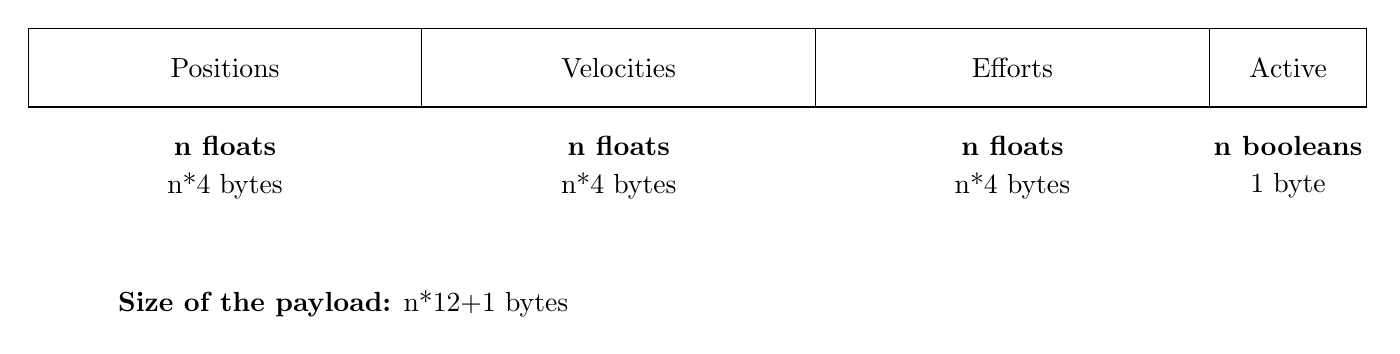
\begin{tikzpicture}

\draw (0,0) rectangle (17,1);
\draw (0,0) rectangle (5,1);
\draw (0,0) rectangle (10,1);
\draw (0,0) rectangle (15,1);

\node at (2.5,0.5) {Positions};
\node at (7.5,0.5) {Velocities};
\node at (12.5,0.5) {Efforts};
\node at (16,0.5) {Active};

\node at (2.5,-0.5) {\textbf{n floats}};
\node at (7.5,-0.5) {\textbf{n floats}};
\node at (12.5,-0.5) {\textbf{n floats}};
\node at (16,-0.5) {\textbf{n booleans}};

\node at (2.5,-1) {n*4 bytes};
\node at (7.5,-1) {n*4 bytes};
\node at (12.5,-1) {n*4 bytes};
\node at (16,-1) {1 byte};

\node at (4,-2.5) {\textbf{Size of the payload:} n*12+1 bytes}; %I have no idea why i need to put 4 as a coordinate for it to not mess up the rest of the figure
\end{tikzpicture}
\caption{Received packet for n motors}
\label{received_packet}
\end{figure}

The structure of the sent packet is shown in figure ~\ref{sent_packet}. To build the packet, the same logic as before is used. The bitcode of the numerical values is copied into a buffer and the buffer is sent.

\begin{figure}
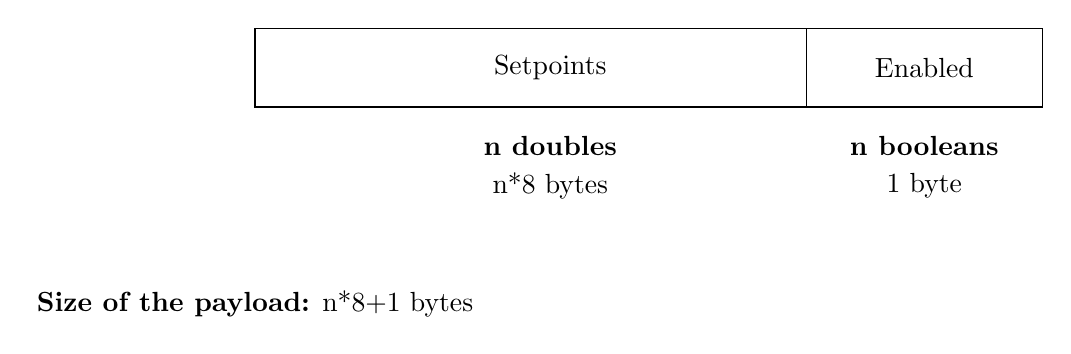
\begin{tikzpicture}

\draw (0,0) rectangle (10,1);
\draw (0,0) rectangle (7,1);

\node at (3.75,0.5) {Setpoints};
\node at (8.5,0.5) {Enabled};

\node at (3.75,-0.5) {\textbf{n doubles}};
\node at (8.5,-0.5) {\textbf{n booleans}};

\node at (3.75,-1) {n*8 bytes};
\node at (8.5,-1) {1 byte};

\node at (0,-2.5) {\textbf{Size of the payload:} n*8+1 bytes}; 
\end{tikzpicture}
\caption{Sent packet for n motors}
\label{sent_packet}
\end{figure}